%%%%%%%%%%%%%%%%%%%%%%%%%%%%%%%%%%%%%%%%%%%%%%%%%%%%%%%%%%%%%%%%%%%%
%% I, the copyright holder of this work, release this work into the
%% public domain. This applies worldwide. In some countries this may
%% not be legally possible; if so: I grant anyone the right to use
%% this work for any purpose, without any conditions, unless such
%% conditions are required by law.
%%%%%%%%%%%%%%%%%%%%%%%%%%%%%%%%%%%%%%%%%%%%%%%%%%%%%%%%%%%%%%%%%%%%

\documentclass{beamer}  
\usetheme[faculty=fi]{fibeamer}
\usepackage[utf8]{inputenc}
\usepackage[
  main=english
]{babel}        %% typeset as follows:
%%
%%   \begin{otherlanguage}{czech}   ... \end{otherlanguage}
%%   \begin{otherlanguage}{slovak}  ... \end{otherlanguage}
%%
%% These macros specify information about the presentation
\title{Cache-Oblivious Priority Queue and Graph Algorithm Applications} %% that will be typeset on the
\author{Alexandru Furculita}
%% These additional packages are used within the document:
\usepackage{ragged2e}  % `\justifying` text
\usepackage{booktabs}  % Tables
\usepackage{tabularx}
\usepackage{tikz}      % Diagrams
\usetikzlibrary{calc, shapes, backgrounds}
\usepackage{amsmath, amssymb}
\usepackage{url}       % `\url`s
\usepackage{listings}  % Code listings
\frenchspacing
\begin{document}
  \frame{\maketitle}

  \AtBeginSection[]{% Print an outline at the beginning of sections
    \begin{frame}<beamer>
      \frametitle{Summary}
      \tableofcontents[currentsection]
    \end{frame}}

  \begin{darkframes}
    \section{Background and previous results}
    
    \subsection{I/O Model or external-memory model}
    \begin{frame}{I/O Model or external-memory model}
        \textbf{Memory architecture:}
        \begin{itemize}
            \item Internal memory of size \textit{\textbf{M}} and,
            \item Arbitrarily large external memory partitioned into blocks of size \textit{\textbf{B}}
        \end{itemize}
      	\bigskip
        \textbf{Efficiency measure:} the number of \textit{memory transfers}, the number of blocks transfered between the two levels of memory\\\bigskip
        \textbf{Limitations:}
        \begin{itemize}
            \item Parameters \textit{\textbf{B}} and \textit{\textbf{M}} must be known
            \item Does not handle multiple memory levels
            \item Does not handle dynamic \textbf{\textit{M}}
        \end{itemize}
    \end{frame}

    \subsection{Cache-oblivious model}
    \begin{frame}{Cache-oblivious model}
        \begin{itemize}
            \item Design and analyze algorithms in the I/O model, but without having the size of the memory and of the blocks as explicit parameters
            \item Analyze in the I/O model for optimal off-line cache replacement strategy: If the main memory is full, the ideal block in main memory is elected for replacement based on the future characteristics of the algorithm
        \end{itemize}
        \bigskip
        \textbf{Advantages:}
        \begin{itemize}
            \item Optimal on arbitrary level optimal on all levels
            \item Portability: \textbf{B} and \textbf{M} not hard-wired into algorithm
            \item Dynamic changing parameters
        \end{itemize}
    \end{frame}

	\subsection{Priority queues}
    \begin{frame}{Priority queues}
        \begin{itemize}
            \item Maintains a set of elements each with a priority (or key) under the operations insert, delete, and deletemin
            \item Analyze in the I/O model for optimal off-line cache replacement strategy: If the main memory is full, the ideal block in main memory is elected for replacement based on the future characteristics of the algorithm
        \end{itemize}
    \end{frame}
    
	\subsection{Priority queues in I/O Model}
    \begin{frame}{Priority queues in I/O Model}
        \begin{block}{Problem}
        Sort \textbf{\textit{N}} elements using an \(O(\log_B N)\) priority queue closer to optimal solution.
      \end{block}
      \bigskip
      The normal algorithms are a factor of \(\frac{\log_B N}{\log_\frac{M}{B} \frac{N}{B}}\) from optimal
    \end{frame}
    
	\subsection{I/O efficient graph algorithms}
    \begin{frame}{I/O efficient graph algorithms}
        \begin{block}{Problem}
        Develop I/O-efficient algorithms for:
        \begin{itemize}
        \item list ranking
        \item Euler Tour
        \item BFS
        \item DFS
        \end{itemize}
      \end{block}
    \end{frame}

	\section{Optimal Cache-Oblivious Priority queues}
    \subsection{Structure}
    \begin{frame}{Optimal Cache-Oblivious Priority queues}
    \framesubtitle{Levels}
    \begin{itemize}
    \item consists of \(\Theta(\log \log N)\) levels of size \(N\) to a constant \(c\)
    \item the size of a level corresponds to the number of elements that can be stored within it
    \end{itemize}
    \end{frame}

    \begin{frame}{Optimal Cache-Oblivious Priority queues}
    \framesubtitle{Buffers}
    A level consists of two levels:
    \begin{itemize}
    \item \textit{up buffer}: only one, can store up to \(X\) elements
    \item \textit{down buffers:} at most \(X^\frac{1}{3}\) such buffers, each containing between \(\frac{1}{2}X^\frac{2}{3}\) and \(2X^\frac{2}{3}\)
    \end{itemize}
    \bigskip
    Three invariants about the relationships between the elements if buffers of various levels are maintained:
    \begin{itemize}
    \item At level \textit{X}, elements are sorted among the down buffers
    \item At level \textit{X}, the elements in the down buffers have smaller keys than the elements in the up buffer
    \item The elements in the down buffers at level \textit{X} have smaller keys than the elements in the down buffers at the next higher level
    \end{itemize}
    \end{frame}

    \begin{frame}{Optimal Cache-Oblivious Priority queues}
    \framesubtitle{Layout}
         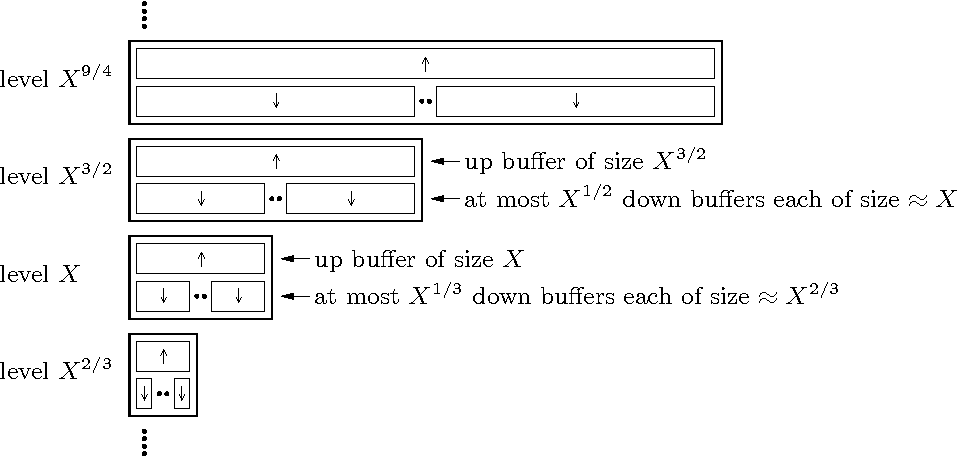
\includegraphics[width=\textwidth]{resources/queue}
    \end{frame}
    
    \subsection{Operations}

    \begin{frame}{Operations}
    \framesubtitle{Push}
    \begin{itemize}
    \item Inserts \textit{X} elements into level \(X^\frac{3}{2}\)
    \item Can be performed in \(O(X^\frac{1}{2} + \frac{X}{B}\log_\frac{M}{B} \frac{X}{B})\) memory transfers amortized
    \end{itemize}
    \end{frame}

    \begin{frame}{Operations}
    \framesubtitle{Pull}
    \begin{itemize}
    \item Removes the \textit{X} elements with smallest keys from level \(X^\frac{3}{2}\) and returns them in sorted order
    \item Can be performed in \(O(1 + \frac{X}{B}\log_\frac{M}{B} \frac{X}{B})\) memory transfers amortized
    \end{itemize}
    \end{frame}

    \begin{frame}{Operations}
    \begin{block}{Total cost}
    A set of \textit{N} elements can be maintained in a linear-space cache-oblivious priority queue data structure supporting each insert, deletemin, and delete operation in \(O(\frac{1}{B}\log_\frac{M}{B} \frac{N}{B})\) amortized memory transfers and \(O(\log_2 N)\) amortized computation time.
    \end{block}
    \end{frame}
    
    \subsection{Graph algorithms}
    \begin{frame}{Graph algorithms applications and results}
    Using the cache oblivious priority queue, there can be developed cache oblivious algorithms for several graph problems that uses the same number of memory accesses as a cache-aware algorithm:
    \begin{itemize}
    \item The list ranking, the Euler Tour, BFS, DFS, and centroid decomposition problems on a \textit{V} node list can be solved in \(O(sort(V))\) memory accesses
    \item The DFS or BFS tree of a directed graph can be computed in \(O((V + \frac{E}{B})\log_2 V + sort(E)\) memory accesses.
    \item The BFS tree of an undirected graph can be computed cache-obliviously in \(O(V + sort(E)\) memory accesses.
    \end{itemize}
    \end{frame}

    \begin{frame}[label=bibliography]{Bibliography}
      \begin{thebibliography}{9}
        \bibitem{demaine}
            Lars Arge, Michael A. Bender, Erik D. Demaine, Bryan Holland‐Minkley, and J. Ian Munro.
            \emph{An Optimal Cache‐Oblivious Priority Queue and Its Application to Graph Algorithms}.
            Available at \url{http://epubs.siam.org/doi/abs/10.1137/S0097539703428324}.
      \end{thebibliography}
    \end{frame}
  \end{darkframes}
\end{document}
